\chapter{\label{cha:sts_transformers}Adapting Transformers for STS}

Transformers can be considered as the most significant revolution that happened in NLP in recent years. Before the introduction of transformers, Recurrent Neural Networks (RNNs) such as LSTMs and GRUs provided state-of-the-art results in NLP tasks. However, RNNs have major limitations. Firstly, since RNNs process the input text in order, they can forget the content of distant positions in the text. As a result, RNNs do not provide good results for long sequences. Secondly, RNNs process the input text, word by word. Therefore, parallelising the work for processing sentences in RNNs is challenging. Transformers can address both of these limitations in RNNs through the attention mechanism \autocite{NIPS2017_3f5ee243}.   


Transformers were first introduced in \textcite{NIPS2017_3f5ee243}, where the authors used a transformer architecture for the sequence to sequence tasks such as machine translation. They show that an architecture with only attention mechanisms and without any RNNs can improve the results in the sequence to sequence tasks. The first notable research in using transformers for language modelling was OpenAI GPT \autocite{radford2018improving}. OpenAI GPT adapts a pre-training followed by a fine-tuning scheme which means that once pre-trained, it can be fine-tuned to a large number of downstream NLP tasks such as text classification, named entity recognition etc. However, the first breakthrough in using transformer models for language modelling happened with the introduction of BERT \autocite{devlin-etal-2019-bert}. As we explain in Section \ref{sec:transformers_related}, BERT employs a masked language modelling (MLM) objective, which brings improvements over OpenAI GPT. Later, different variants of BERT were proposed by the NLP community. We explain some of these models that we used in this chapter in Section \ref{sec:transformers_related}. All of these transformer models follow the same fine-tuning scheme of BERT.


Transformer models, which we have experimented with in this chapter, use special tokens to obtain a single contiguous sequence for each input sequence. Specifically, the first token is always a special classification token (\textsc{[CLS]}), and sentence pairs are separated using a special token (\textsc{[SEP]}). The final hidden state of \textsc{[CLS]}  is used for the sentence-level fine-tuning tasks such as text classification \autocite{10.1007/978-3-030-32381-3_16, ranasinghe-hettiarachchi-2020-brums}, and the final hidden state of each token is used for the token-level fine-tuning tasks such as named entity recognition \autocite{taher-etal-2019-beheshti, ranasinghe-etal-2021-wlv,jia-etal-2020-entity}. The fine-tuning scheme in transformers is usually simple. For example, transformer models can be adapted to text classification tasks by adding a softmax layer on top of \textsc{[CLS]} token. Furthermore, the fine-tuning scheme is very efficient as the parameters in the transformer model are already optimised in the pre-training process. Therefore, transformer models have been prevalent and successful in many NLP tasks \autocite{devlin-etal-2019-bert}. 

Since the fine-tuning scheme is very efficient in transformers, they can be optimised with less training data. Therefore, given the amount of human labour required to produce datasets for STS, transformers can provide an ideal solution for STS. Furthermore, the state-of-the-art results transformers produced for different NLP tasks motivated us to explore transformers in STS. In this chapter, we experiment with different transformers models in a variety of STS datasets.
 
We address four research questions in this chapter:

\textbf{RQ1:} How well do the existing state-of-the-art transformer models perform in the STS task? 

\textbf{RQ2:} Can the method improve with the transfer learning and data augmentation techniques?

\textbf{RQ3:} Can the transformer model be easily adapted to different languages?

\textbf{RQ4:} How well do the proposed transformer models perform in a different domain? 

The main contributions of this chapter are as follows.

\begin{enumerate}
\item We evaluate five popular transformer models in three English STS datasets. We compare the results with the previous STS methods and show that transformer-based STS methods outperform all the other STS methods we have experimented with in this thesis.

\item We propose further enhancements to the architecture using transfer learning and data augmentation.   

\item We evaluate how well the transformer models perform on STS datasets in different languages and domains. 

\item The code and the pre-trained models are publicly available to the community\footnote{The public GitHub repository is available on \url{https://github.com/tharindudr/STS-Transformers}.}. We have published the code as a Python library \footnote{The developed python library is available on \url{https://pypi.org/project/ststransformers/}.} and by the time of writing this chapter, it has more than 3,000 downloads from the community. 

\end{enumerate}

The rest of this chapter is organised as follows. Section \ref{sec:transformers_related} describes the pre-trained transformer models used in this chapter. Section \ref{sec:transformer_method} discusses the architecture and \ref{sec:transformer_english} shows the experiments conducted with three English STS datasets. Sections \ref{sec:transformer_transfer} and \ref{sec:transformer_aug} provide more experiments to improve the results. Experiments done with other languages and domains are shown in Sections \ref{sec:transformer_multilingual} and \ref{sec:transformer_domain}. Section \ref{sec:transformer_siamese} discusses the recent developments carried out with integrating transformers into Siamese architectures, addressing a key issue in using transformers in STS. The chapter finishes with conclusions and ideas for future research directions in transformers. 

\section{Related Work}
\label{sec:transformers_related}
As we mentioned before, after the introduction of BERT \autocite{devlin-etal-2019-bert}, many variants of different transformer models have been proposed by adding minor modifications to the original BERT transformer. Usually, these modifications have resulted in improvements in the fine-tuning scheme for the downstream NLP tasks. Expecting a similar behaviour for the STS task, we evaluated the following transformer models for the experiments in this chapter.

\paragraph{BERT} \autocite{devlin-etal-2019-bert} proposes an MLM objective, where some of the tokens of the input sequence are randomly masked, and the objective is to predict these masked positions, taking the corrupted sequence as input. BERT applies a Transformer encoder to attend to bi-directional contexts during pre-training. In addition, BERT uses a next-sentence-prediction (NSP) objective. Given two input sentences, NSP predicts whether the second sentence is the next sentence of the first sentence. The NSP objective aims to improve the tasks which require reasoning over sentence pairs, such as question answering and natural language inference. 

\paragraph{RoBERTa} \autocite{liu2019roberta} makes a few changes to the BERT architecture and achieves substantial improvements. These changes include: (1) Training the model longer with larger batches and more data; (2) Removing the NSP objective; (3) Training on longer sequences; (4) Dynamically changing the masked positions during pre-training. The authors show that these changes lead to significant improvements in the downstream NLP tasks.

\paragraph{ALBERT} \autocite{Lan2020ALBERT} proposes two parameter-reduction techniques (factorised embedding parameterisation and cross-layer parameter sharing) to lower memory consumption and speed up training. Furthermore, ALBERT \autocite{Lan2020ALBERT} shows that the NSP objective in BERT lacks difficulty, as the negative examples are created by pairing segments from different documents, which mixes topic prediction and coherence prediction into a single task. Instead of that, ALBERT uses a sentence-order prediction (SOP) objective. SOP obtains positive examples by taking out two consecutive segments and negative examples by reversing the order of two consecutive segments from the same document. The results show that ALBERT provides better results than BERT in many downstream NLP tasks.


\paragraph{ELECTRA} Compared to BERT, ELECTRA \autocite{Clark2020ELECTRA} proposes an effective pre-training method. Instead of corrupting some positions of inputs with [MASK], ELECTRA replaces some tokens of the inputs with their plausible alternatives sampled from a small generator network. ELECTRA trains a discriminator to predict whether the generator replaced each token in the corrupted input or not. The pre-trained discriminator can then be used in downstream tasks for fine-tuning, improving upon the pre-trained representation learned by the generator.ed in downstream tasks for fine-tuning, improving upon the pre-trained representation learned by the generator.

\paragraph{XLNET} \autocite{yang2019xlnet} addresses a key weakness in BERT pre-training. \textcite{yang2019xlnet} show that the symbols such as \textsc{[MASK]} that BERT introduces during pre-training cause a discrepancy between pre-training and fine-tuning as they never occur in real data. Therefore, XLNET proposes a new auto-regressive method based on permutation language modelling (PLM) \autocite{JMLR:v17:16-272} without introducing new symbols. 

Upon the introduction, these transformer models are evaluated in many downstream NLP tasks, including STS. However, there is no comprehensive study on STS using the transformers in large and small STS datasets, transfer learning, data augmentation, multilingual STS, etc., which we do in this chapter.

\section{Transformer Architecture for STS}
\label{sec:transformer_method}

\begin{figure}[ht]
	\centering
	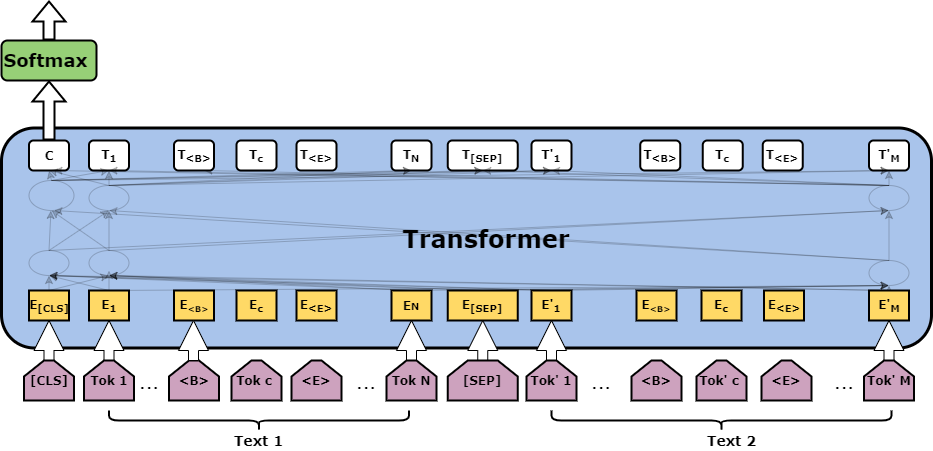
\includegraphics[scale=0.4]{figures/semantic_textual_similarity/transformers/STSTransformers.png}
	\caption[Architecture for using Transformers in STS]{Architecture for using Transformers in STS.}
	\label{fig:sts_transformers}
\end{figure}

The transformer architecture for STS is shown in Figure \ref{fig:sts_transformers}. The input of this model is a concatenation of the two sentences, separated by the \textsc{[SEP]} token. Then the output of the \textsc{[CLS]} token is used as the input of a softmax layer that predicts the similarity of the two sentences. We used the mean-squared-error loss as the objective function. For the configurations, we used a batch-size of eight, Adam optimiser with a learning rate $2\mathrm{e}^{-5}$, and a linear learning rate warm-up over 10\% of the training data. During the training process, the parameters of the transformer and the parameters of the subsequent layers were updated. The models were trained using only training data. Furthermore, they were evaluated while training after every 100 batches, using an evaluation set that had one-fifth of the instances in training data. We performed early stopping if the evaluation loss did not improve over ten evaluation steps. All the models were trained for three epochs. As these transformer models are computationally expensive, we used an Nvidia Tesla T4 GPU for the training process. We have kept these configurations the same for all the experiments to ensure consistency between all the experiments. The implementation is based on PyTorch \autocite{NEURIPS2019_9015} and HuggingFace \autocite{wolf-etal-2020-transformers}.


\section{Exploring Transformers in English STS}
\label{sec:transformer_english}
We evaluated all the transformer variations mentioned before, in three English STS datasets we introduced in \ref{cha:sts_introduction}; SICK, STS 2017 and QUORA. All of the transformer models we experimented have several models that supports English (e.g.\ \textit{bert-large-cased} \& \textit{bert-base-cased} for BERT, \textit{albert-xxlarge-v2} \& \textit{albert-base-v2} for ALBERT), and usually the large models outperform the smaller models in downstream tasks. Therefore, we used the largest possible model that our GPU setup can load with each transformer type; \textit{bert-large-cased} for BERT \autocite{devlin-etal-2019-bert}, \textit{albert-large-v2} for ALBERT \autocite{Lan2020ALBERT}, \textit{roberta-large} for RoBERTa \autocite{liu2019roberta}, \textit{google/electra-large-discriminator} for ELECTRA \autocite{Clark2020ELECTRA} and \textit{xlnet-large-cased}  \autocite{yang2019xlnet} for XLNET. All of these models are available in HuggingFace \autocite{wolf-etal-2020-transformers} model hub\footnote{Models are available on \url{https://huggingface.co/models}}.

We trained the transformer models on the training sets of these datasets and evaluated on the testing sets. The results for the SICK, STS2017 and QUORA are shown in Tables \ref{tab:sick_transformers}, \ref{tab:sts_transformers} and \ref{tab:quora_transformers}, respectively. 

\begin{table*}[htb]
	%\footnotesize
	\centering
	\scalebox{0.95}{
		\begin{tabular}{|l|cc|}
			\hline
			\textbf{Model} & $\bm{\rho}$   & $\bm{\tau}$     
			\\ \hline
			\textit{BERT}                  
			& 0.881 & 0.826  \\
			\textit{ALBERT}                  
			& 0.886 & 0.829  \\
			\textit{RoBERTa}                  
			& 0.892$^{\dagger}$ & 0.834$^{\dagger}$  \\
			\textit{ELECTRA}                  
			& 0.872 & 0.819  \\
			\textit{XLNET}                  
			& 0.879 & 0.821  \\
			\hline
		\end{tabular}
	}
	\caption[Results for SICK with Transformer Models]{Results for SICK dataset with different variants of transformer models. For each variant, Pearson Correlation ($\bm{\rho}$) and Spearman Correlation ($\bm{\tau}$) are reported between the predicted values and the gold labels of the test set. The best result from all of the variations is marked with ${\dagger}$.}  
	\label{tab:sick_transformers}
\end{table*}


\begin{table*}[htb]
	%\footnotesize
	\centering
	\scalebox{0.95}{
		\begin{tabular}{|l|cc|}
			\hline
			\textbf{Model} & $\bm{\rho}$   & $\bm{\tau}$     
			\\ \hline
				\textit{BERT}                  
		& 0.889 & 0.858  \\
		\textit{ALBERT}                  
		& 0.874 & 0.852  \\
		\textit{RoBERTa}                  
		& 0.895$^{\dagger}$ & 0.861$^{\dagger}$  \\
		\textit{ELECTRA}                  
		& 0.873 & 0.849  \\
		\textit{XLNET}                  
		& 0.868 & 0.843  \\
			\hline
		\end{tabular}
	}
	\caption[Results for STS 2017 with Transformers]{Results for STS 2017 dataset with different variants of Transformers. For each variant, Pearson Correlation ($\bm{\rho}$) and Spearman Correlation ($\bm{\tau}$) are reported between the predicted values and the gold labels of the test set. The best result from all of the variations is marked with ${\dagger}$. }  
	\label{tab:sts_transformers}
\end{table*}


\begin{table*}[htb]
	%\footnotesize
	\centering
	\scalebox{0.95}{
		\begin{tabular}{|l|c|}
			\hline
			\textbf{Model} & RMSE     
			\\ \hline
			\textit{BERT}                  
			& 0.349   \\
			\textit{ALBERT}                  
			& 0.354   \\
			\textit{RoBERTa}                  
			& 0.359   \\
			\textit{ELECTRA}                  
			& 0.353   \\
			\textit{XLNET}                  
			& 0.346$^{\dagger}$   \\
			\hline
		\end{tabular}
	}
	\caption[Results for QUORA with Transformers]{Results for QUORA dataset with different variants of Transformers. For each variant, Root Mean Squared Error (RMSE) reported between the predicted values and the gold labels of the test set. The best result from all of the variations is marked with ${\dagger}$. }  
	\label{tab:quora_transformers}
\end{table*}

As can be seen in Tables \ref{tab:sick_transformers} and \ref{tab:sts_transformers}, for the SICK and STS 2017 datasets, RoBERTa outperformed other transformer models. Since SICK and STS 2017 are smaller datasets, the optimised nature of RoBERTa is beneficial. The QUORA dataset, which is larger than the SICK and STS 2017, \textit{XLNET}  outperforms other transformer models. However, from the results, there is no clear indication of which transformer model would perform best in a particular dataset other than the fact that the \textit{RoBERTa} performs slightly better in smaller datasets. It should be noted that all of the transformers perform on par with each other. 

In the initial experiments, we noticed that the transformer models are susceptible to the random seed\footnote{A random seed is used to configure the starting weights in a neural network. Keeping the random seed constant in the experiments removes the variation due to this randomness, making it easier to interpret the effects of other design changes such as hyperparameter values.} of the experiments \autocite{zhang2021revisiting}. Changing the random seed led to different results. To minimise this effect from the random seed, we conducted experiments for five different random seeds. We took the mean of these experiments as the final results, which is the value reported in Tables \ref{tab:sick_transformers}, \ref{tab:sts_transformers} and \ref{tab:quora_transformers}. We noticed that doing many experiments with different random seeds reduced the variance of the final result. 

With this, we answer our \textbf{RQ1}: transformers can be successfully adapted in the STS task, and they produce good results in all the datasets. For the smaller datasets, \textit{RoBERTa} performed slightly better than other transformer models. Furthermore, we recommend conducting more experiments with different random seeds to minimise the variance.


\subsection{Impact of Transfer Learning}
\label{sec:transformer_transfer}
Similar to the \textit{Siamese neural networks} in Chapter \ref{cha:sts_siamese_neural_networks}, we explored the impact of transfer learning  in STS, with transformers. We saved the weights of the transformers models trained on each STS dataset; SICK, STS 2017 and QUORA. We specifically used the two models that performed best in these datasets; RoBERTa and XLNET. We again initiated training for each dataset; however, rather than training the transformer models from scratch, we used the weights of the models trained on a different STS dataset. We compared these transfer learning results to the results we got from training the model from scratch. Similar to the \textit{Siamese neural network} experiments, we conducted this transfer learning experiment only on the STS2017 and SICK datasets since the QUORA dataset is already large and transfer learning from a smaller dataset to a larger dataset is nonsensical.


\begin{table*}[htb]
	%\footnotesize
	\centering
	\scalebox{0.95}{
		\begin{tabular}{|l|c|c|}
			\hline
			\textbf{Start Model} & STS2017 & SICK      
			\\ \hline
			\textit{STS2017$_{RoBERTa}$}                  
			& 0.895 & \textcolor{gray}{(+0.009)} \\
			\textit{STS2017$_{XLNET}$}                     
			& 0.868 & \textcolor{gray}{(+0.011)}  \\
			\hline
			\textit{SICK$_{RoBERTa}$}                     
			& \textcolor{gray}{(+0.008)} & 0.892 \\
			\textit{SICK$_{XLNET}$}                     
			& \textcolor{gray}{(+0.013)} & 0.879 \\
			\hline
			\textit{QUORA$_{RoBERTa}$}                     
			& \textcolor{gray}{(-0.025)}  &  \textcolor{gray}{(-0.021)}    \\
			\textit{QUORA$_{XLNET}$}                     
			& \textcolor{gray}{(-0.039)} &  \textcolor{gray}{(-0.043)}    \\
			\hline
		\end{tabular}
	}
	\caption[Results for transfer learning with Transformers]{Results for transfer learning with different Transformers. For each transfer learning experiment we show the difference between with and without transfer learning. Non-grey values are the results of the experiments without transfer learning which we showed in the previous section. For ease of visualisation we only report the Pearson correlation ($\bm{\rho}$).}  
	\label{tab:transfer_transformers}
\end{table*}

As can be seen in Table \ref{tab:transfer_transformers}, when we performed transfer learning from STS2017 $\Rightarrow$ SICK and SICK $\Rightarrow$ STS2017 the results improve. This shows that transfer learning can improve the results of transformers. However, similar to the \textit{Siamese neural networks}, when we performed transfer learning from QUORA $\Rightarrow$ STS2017 and QUORA $\Rightarrow$ SICK, the results did not improve, in fact, they decrease. Therefore, we can assume that performing transfer learning from a very different dataset, is not beneficial in transformers. 

Therefore, we can conclude that transfer learning can improve the results for transformers in STS. However, the transfer learning dataset should be picked carefully, taking the similarity of the two datasets into consideration, rather than only considering the size of the dataset.


\subsection{Impact of Data Augmentation}
\label{sec:transformer_aug}
Since the transformer models have provided better results with more training data, we experimented with the impact of data augmentation on the transformer models. Similar to the \textit{Siamese neural networks} in Chapter \ref{cha:sts_siamese_neural_networks}, we employed thesaurus-based augmentation in which 10,000 additional training examples are generated by replacing random words with one of their synonyms in Wordnet \autocite{10.1145/219717.219748}. We specifically used the two models that performed best with the bigger dataset and smaller dataset; \textit{RoBERTa} and \textit{XLNET}. Since using transfer learning improved the results in the previous experiment, we trained the augmented training set on the transferred models; models trained on STS2017 for the SICK experiments and models trained on SICK for the STS2017 experiments. The results are shown in Table \ref{tab:augmentation_transformers}. 

\begin{table*}[htb]
	%\footnotesize
	\centering
	\scalebox{0.95}{
		\begin{tabular}{|c|c|c|}
			\hline
			\textbf{Dataset} &	\textbf{Start Model} &  $\bm{\rho}$      
			\\ \hline
			\multirow{ 2}{*}{\textit{SICK}}	& \textit{STS2017$_{RoBERTa}$}                  
			& \textcolor{gray}{(+0.012)} \\
			&	\textit{STS2017$_{XLNET}$}                     
			& \textcolor{gray}{(+0.011)}  \\
			\hline
			\multirow{ 2}{*}{\textit{STS2017}}  & \textit{SICK$_{RoBERTa}$}                     
			& \textcolor{gray}{(+0.014)}  \\
			& \textit{SICK$_{XLNET}$}                     
			& \textcolor{gray}{(+0.013)} \\
			\hline
		\end{tabular}
	}
	\caption[Results for data augmentation with Transformers]{Results for data augmentation with different transformers. For each data augmentation experiment we show the difference between with dat augmentation and without data augmentation. For ease of visualisation we only report the Pearson correlation ($\bm{\rho}$).}  
	\label{tab:augmentation_transformers}
\end{table*}

As can be seen in Table \ref{tab:augmentation_transformers}, data augmentation improved the results of all the experiments with transformers. However, even with the additional 10,000 training instances, \textit{RoBERTa} outperformed \textit{XLNET}. We can conclude that simple data augmentation techniques can improve the performance of transformers in the STS task. From the experiments we conducted, our best results for both the STS2017 and SICK datasets were produced by \textit{RoBERTa} when combined with transfer learning and data augmentation.


These observations answer our \textit{RQ2} in this Chapter; we can use transfer learning and simple data augmentation techniques to improve the results of transformers in STS. 

\begin{table*}[htb]
	%\footnotesize
	\centering
	\scalebox{0.95}{
		\begin{tabular}{|l|c|}
			\hline
			\textbf{Model} & $\bm{\rho}$      
			\\ \hline
			\textcite{jimenez-etal-2014-unal} & 0.807 \\
			\textcite{bjerva-etal-2014-meaning} & 0.827 \\
			\textcite{zhao-etal-2014-ecnu-one} & 0.841 \\
			\textit{Siamese GRU} & 0.882  \\
			\textit{RoBERTa} & 0.920  \\
			\hline
		\end{tabular}
	}
	\caption[Results comparison for SICK with leader board results including transformers]{Results for the SICK dataset with different transformer models. For each variant, Pearson Correlation ($\bm{\rho}$) is reported between the predicted values and the gold labels of the test set.}  
	\label{tab:sick_transformers_all}
\end{table*}

\begin{table*}[htb]
	%\footnotesize
	\centering
	\scalebox{0.95}{
		\begin{tabular}{|l|c|}
			\hline
			\textbf{Model} & $\bm{\rho}$      
			\\ \hline
			\textcite{tian-etal-2017-ecnu} & 0.851 \\
			\textcite{maharjan-etal-2017-dt} & 0.854 \\
			\textcite{cer-etal-2017-semeval}  & 0.855   \\
			\textit{Siamese GRU} & 0.862  \\
			\textit{RoBERTa} & 0.915  \\
			\hline
		\end{tabular}
	}
	\caption[Results comparison for STS2017 with leader board results]{Results for the STS2017 dataset with different variants of Siamese Neural Network. For each variant, Pearson Correlation ($\bm{\rho}$) is reported between the predicted values and the gold labels of the test set.  }  
	\label{tab:sts_transformers_all}
\end{table*}

Furthermore, we compared the results of the best transformer model with the best results submitted to the competitions \autocite{cer-etal-2017-semeval, marelli-etal-2014-semeval}, and with the supervised and unsupervised STS methods, we have experimented in this thesis. As can be seen in Tables \ref{tab:sick_transformers_all} and \ref{tab:sts_transformers_all}, \textit{RoBERTa} outperforms the best system submitted to both competitions. It also outperforms the unsupervised and supervised STS methods we have explored in this thesis, including \textit{Siamese neural networks}. Therefore, we can conclude that transformers are the current state-of-the-art for English STS.

\section{Portability to Other Languages}
\label{sec:transformer_multilingual}
Similar to the other STS methods we have experimented with in this thesis, we evaluated transformers in Arabic STS and Spanish STS datasets introduced in Chapter \ref{cha:sts_introduction}. Transformers have the advantage that they do not rely on language-dependent features.  As a result, the approach is easily portable to other languages, given the availability of the pre-trained transformer models in that particular language. The transformer models, we used are AraBERT and AraELECTRA for Arabic which were trained on Arabic Wikipedia dump, the 1.5B words Arabic Corpus \autocite{elkhair201615}, the OSCAR corpus \autocite{ortiz-suarez-etal-2020-monolingual} and the OSIAN Corpus \autocite{zeroual-etal-2019-osian} using original BERT and ELECTRA architectures explained in Section \ref{sec:transformers_related}\footnote{More details about the models and download links are available on \url{https://github.com/aub-mind/arabert}}. Both of these models use Farasa segmentation as a pre-processing step \autocite{abdelali-etal-2016-farasa}. For Spanish, we used BETO; a Spanish BERT model \autocite{CaneteCFP2020} trained on Spanish Unannotated Corpora\footnote{Corpora is available on \url{https://github.com/josecannete/spanish-corpora}} using the original BERT architecture\footnote{More details about BETO is available on \url{https://github.com/dccuchile/beto}}. Additionally, for both languages, we used the "BERT-Base, Multilingual Cased" model \autocite{devlin-etal-2019-bert}, which is trained on the top 100 languages with the largest Wikipedias that includes Arabic and Spanish languages.

The results are shown in Tables \ref{tab:arabic_transformers_all} and \ref{tab:spanish_transformers_all} for the Arabic and Spanish datasets. We also compared the results of the transformer models with the best methods submitted to the competition \autocite{cer-etal-2017-semeval}, and with the supervised/unsupervised STS methods, we have experimented in this thesis. 


\begin{table*}[htb]
	%\footnotesize
	\centering
	\scalebox{0.95}{
		\begin{tabular}{|l|c|}
			\hline
			\textbf{Model} & $\bm{\rho}$      
			\\ \hline
			\textcite{tian-etal-2017-ecnu} & 0.744 \\
			\textcite{nagoudi-etal-2017-lim} & 0.746 \\
			\textcite{wu-etal-2017-bit}  & 0.754   \\
			\textit{Siamese GRU} & 0.763  \\
			\textit{mBERT} & 0.778\\
			\textit{AraElectra} & 0.791\\
			\textit{AraBERT} & \textbf{0.794} \\
			\hline
		\end{tabular}
	}
	\caption[Results comparison for Arabic STS with leader board results]{Results for the Arabic STS dataset with different transformers. For each variant, Pearson Correlation ($\bm{\rho}$) is reported between the predicted values and the gold labels of the test set. }  
	\label{tab:arabic_transformers_all}
\end{table*}


\begin{table*}[htb]
	%\footnotesize
	\centering
	\scalebox{0.95}{
		\begin{tabular}{|l|c|}
			\hline
			\textbf{Model} & $\bm{\rho}$   \\  
			\hline
			\textcite{hassan-etal-2017-fcicu} & 0.848 \\
			\textcite{wu-etal-2017-bit} &  0.850 \\
			\textcite{tian-etal-2017-ecnu} & 0.855 \\
			\textit{Siamese GRU} & 0.863  \\
			\textit{mBERT} & 0.884  \\
			\textit{BETO} & \textbf{0.890}  \\
			\hline
		\end{tabular}
	}
	\caption[Results comparison for Spanish STS with leader board results]{Results for the Spanish STS dataset with different variants of Siamese Neural Network. For each variant, Pearson Correlation ($\bm{\rho}$) is reported between the predicted values and the gold labels of the test set. }  
	\label{tab:spanish_transformers_all}
\end{table*}

As can be seen in the results transformer based STS method outperformed all the other supervised and unsupervised STS models in both languages and outperforms the top systems of the competition in both languages. From the experimented pre-trained transformer models, language specific models like BETO, AraBERT outperformed general multilingual models.  Therefore, we can conclude that  transformers are currently the state-of-the-art for Arabic and Spanish STS too. Furthermore, it should be noted that it is very easy to adapt transformers in a different language. We only changed the pre-trained model to the new language and performed the training. 

This answers our \textbf{RQ3:}, the transformers can be successfully adapted in different languages by changing the pre-trained model and the training dataset. They produce state-of-the-art results in STS.

\section{Potability to Other Domains}
\label{sec:transformer_domain}
To answer our \textbf{RQ4}; how well the proposed transformer models can be applied in STS tasks in different domains, we evaluated our method on the Bio-medical STS dataset explained in Chapter \ref{cha:sts_introduction} (BIOSSES). As we mentioned previously, the Bio-medical STS dataset does not have a training set. Therefore, we had to follow a transfer learning strategy to evaluate transformers on the Bio-medical STS dataset. Similar to \textit{Siamese neural network} experiments in Chapter \ref{cha:sts_siamese_neural_networks}, we used the pre-trained English STS transformer models and performed inference on the Bio-medical STS dataset. 

For this transfer learning strategy, we considered two pre-trained transformer models; \textit{bert-large-cased} \autocite{devlin-etal-2019-bert} (\textit{BERT}) which we used in the English STS experiments and, BioBERT \autocite{10.1093/bioinformatics/btz682} which has trained BERT on PubMed abstracts\footnote{More details and the model are available on \url{https://github.com/dmis-lab/biobert}}.

\begin{table*}[htb]
	%\footnotesize
	\centering
	\scalebox{0.95}{
		\begin{tabular}{|l|c|c|}
			\hline
			\textbf{Data} & \textbf{BERT} & \textbf{BioBERT}      
			\\ \hline
			\textit{STS2017}                  
			& 0.663 & 0.763 \\
			\textit{SICK}                     
			& 0.658 & 0.751  \\
			\textit{QUORA}                     
			& 0.612 & 0.682 \\
			\hline
		\end{tabular}
	}
	\caption[Results for transfer learning with transformers in the BIOSSES dataset]{Results for transfer learning with transformers in the BIOSSES dataset. Two considered pre-trained transformer models are textbf{BERT} and \textbf{BioBERT}. For ease of visualisation we only report the Pearson correlation ($\bm{\rho}$).}  
	\label{tab:transfer_transformers_biosses}
\end{table*}


As can be seen in the Table \ref{tab:transfer_transformers_biosses}, transformers provided satisfactory results in Bio-medical STS. We got the best result from transformers when trained on STS 2017 using BioBERT. Furthermore, there was a clear improvement when the English STS model was trained using BioBERT rather than general BERT. This may be because most of the Bio-medical words that appear in the BIOSSES dataset are out of vocabulary in the general BERT model, which can cause problems to the neural network when it observes them in the testing phase. Furthermore, it should be noted that in this experiment, when we performed transfer learning from the QUORA dataset, the results are lower than when we performed transfer learning from SICK or STS 2017. This again can be due to the reason that the SICK and STS 2017 datasets have a similar annotation strategy to the BIOSSES dataset as discussed in Chapter \ref{cha:sts_introduction}. These results are similar to what we observed with \textit{Siamese neural networks} in Chapter \ref{cha:sts_siamese_neural_networks}.

\begin{table*}[htb]
	%\footnotesize
	\centering
	\scalebox{0.90}{
		\begin{tabular}{|l|c|}
			\hline
			\textbf{Model} & $\bm{\rho}$   \\  
			\hline
			\textit{ELMo $\bigoplus$ BERT}  &  0.708 \\
			\textit{Siamese GRU$_{STS2017}$} & 0.719 \\
			\textcite{10.1093/bioinformatics/btx238} & 0.754 \\
			\textit{BioBERT$_{STS2017}$} & 0.763 \\
			\textit{BioSentVec} \autocite{8904728} & 0.810  \\
			\hline
		\end{tabular}
	}
	\caption[Results comparison for BIOSSES with top results and transformers]{Results for the BIOSSES dataset with transformers compared with top results reported for BIOSSES. For each variant, Pearson Correlation ($\bm{\rho}$) is reported between the predicted values and the gold labels of the test set. }  
	\label{tab:biosses_transformers_all}
\end{table*}

Furthermore, we compared our results with the best results reported for the dataset. The results are shown in Table \ref{tab:biosses_transformers_all}. The best model we had in Table \ref{tab:transfer_transformers_biosses} which is based on BioBERT when trained on STS2017, is represented as \textit{BioBERT$_{STS2017}$}. As shown in the results, our method provides satisfactory results when compared to the best approaches. Also, it outperforms the GRU based \textit{Siamese neural network} architecture we experimented in Chapter \ref{cha:sts_siamese_neural_networks} using the same transfer learning strategy. However, the unsupervised method we experimented with in Chapter \ref{cha:sts_sentence_encoders} with BioSentVec \autocite{8904728} comfortably outperformed the transformer-based STS method we experimented with in this Chapter.

With these observations, we can answer our \textbf{RQ4}: \textit{How well do the proposed transformer models perform in a different domain?}. The transformers can be adapted to STS tasks in different domains by changing the pre-trained transformer model. However, without a proper training set, the results are not strong. This is a common observation we had for supervised STS methods in this thesis.



\section{Recent Developments: \\ Siamese Transformers}
\label{sec:transformer_siamese}

\begin{figure}[ht]
	\centering
	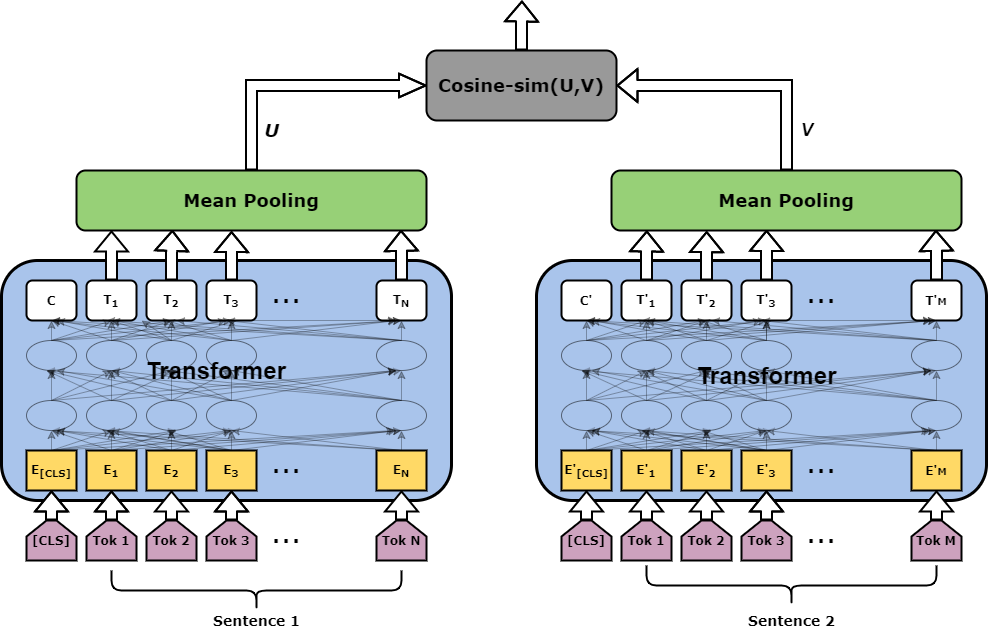
\includegraphics[scale=0.35]{figures/semantic_textual_similarity/transformers/sentence-bert.png}
	\caption[Architecture for using Siamese Transformers in STS]{Architecture for using Siamese Transformers in STS.}
	\label{fig:siamese_transformers}
\end{figure}

As we observed in previous experiments, transformers are state-of-the-art in supervised STS. However, to predict the similarity in test time, both sentences must be fed into the network. Two sentences are passed to the transformer network, and the similarity is predicted. However, this setup is unsuitable for various text similarity tasks. For example, finding the sentence pair with the highest similarity in a collection of n = 10 000 sentences requires $n \times \frac {(n-1)}{2} = 49,995,000$ inference computations with the default transformer architecture experimented in this chapter. On a modern V100 GPU, this requires about 65 hours. Similarly, finding the most similar question for a new question from over 40 million existing questions in Quora would require over 50 hours. This massive computational overload is not suitable for many real-world applications \autocite{reimers-gurevych-2019-sentence}.

The obvious solution to this would be to get sentence embeddings from the transformer network. A common approach is to use vector aggregation methods that we already experimented in Chapter \ref{cha:sts_state_of_the_art_methods}. However, we previously showed that these simple, unsupervised vector aggregation-based STS methods are outperformed by sentence encoders that use traditional word embeddings. Therefore, \textcite{reimers-gurevych-2019-sentence} propose a Siamese neural architecture based on transformers. The architecture is shown in Figure \ref{fig:siamese_transformers}, which is similar to the Siamese architectures we experimented in Chapter \ref{cha:sts_siamese_neural_networks}.

This architecture can be trained on an STS dataset. Since this is a Siamese architecture, it can produce sentence embeddings that can be used at the inference time without having both sentences in the network. \textcite{reimers-gurevych-2019-sentence} show that this architecture provides less accuracy than the default transformer architecture in STS tasks. Yet, the results are very compatible and outperform other sentence encoders such as Universal Sentence Encoder and Infersent. Furthermore, it outperforms the word embedding based Siamese neural network architectures experimented in Chapter \ref{cha:sts_siamese_neural_networks}. Therefore, this architecture is the current state-of-the-art Siamese neural network in STS tasks. \textcite{reimers-gurevych-2019-sentence} calculate that the complexity for finding the most similar sentence pair in a collection of 10,000 sentences is reduced from 65 hours with the default architecture to 5 seconds with the Siamese transformer architecture. We can conclude that this architecture is very efficient in many NLP applications where it is required to find similar sentences from a large set of sentences, such as Translation Memories\footnote{More details and the pre-trained models on Siamese transformers are available on \url{https://www.sbert.net/}}.  


\section{Conclusions}
In this chapter, we experimented with utilising state-of-the-art transformers in the STS task. We evaluated the default sentence pair regression architecture on transformers in three English datasets, two non-English datasets and a bio-medical STS dataset. For the smaller STS datasets, we showed that \textit{RoBERTa} outperformed other transformer models. For the larger STS dataset, \textit{XLNET} provided the best result. We showed that we could improve the results with transfer learning and data augmentation techniques. For the three English and two non-English datasets, the transformer-based STS method outperformed all the other supervised and unsupervised STS methods we experimented with in this part of the thesis. Furthermore, they outperformed the best systems submitted for each competition. This shows that the transformers are the current state-of-the-art in supervised STS.

However, in the BIOSSES dataset where it does not have a training set, we used a transfer learning based zero-shot learning when transformers are applied. Even though transformers outperformed other STS methods we experimented such as Siamese neural networks, they could not outperform the sentence vector-based method we experimented with in Chapter \ref{cha:sts_sentence_encoders}. We can conclude that although the transformers can be adapted in different domains by changing the pre-trained model, they do not provide strong results without a proper training set. 

One major limitation in the transformer-based STS method is that it requires to have both sentences in the network at the inference time, which can cause a massive computational overhead for some NLP applications. To overcome this, \textcite{reimers-gurevych-2019-sentence} proposed a Siamese transformer architecture that is capable of providing sentence vectors that can reduce the inference time. Another limitation in the transformers is the pre-trained transformer models are large and can cause problems in real-world applications. As a solution to this, we hope to explore knowledge distillation \autocite{Gou2021} in STS tasks. With knowledge distillation, transformer-based methods can be used as teacher models to train simple student models such as Siamese GRU, which would provide competitive results to transformer-based STS methods but with smaller disk space. 

With this, we conclude Part I of the thesis. We explored numerous STS methods based on word vectors which are easy to adapt in different languages and domains. We evaluated them on different STS datasets and discussed their benefits and limitations in each chapter. We can conclude that transformers are state-of-the-art in supervised STS methods and sentence encoders are state-of-the-art in unsupervised STS methods. Keeping in mind the benefits and limitations of these STS methods, in the following two parts of the thesis, we will employ them in two applications in translation technology; translation memories in Part II and translation quality estimation in Part III.

